\documentclass[a4paper]{llncs}
\usepackage[T1]{fontenc}
\usepackage{mathptmx}
\usepackage{amsmath,amssymb,graphicx,booktabs,url}
\usepackage[hidelinks]{hyperref}
% Register a passive attachment in the PDF's EmbeddedFiles name tree.
% The scientific ZIP includes these sources and deliberately excludes itself.
\newif\ifResearchAttached
\edef\ResearchZipName{\detokenize{R2_Frame_Loss_Research.zip}}
\edef\ResearchZipPath{supplement/\ResearchZipName}
\IfFileExists{\ResearchZipPath}{%
  \ifdefined\pdfobj
    \ifnum\pdfoutput>0
      \immediate\pdfobj stream attr {/Type /EmbeddedFile} file {\ResearchZipPath}%
      \edef\ResearchStream{\the\pdflastobj\space 0 R}%
      \immediate\pdfobj{<< /Type /Filespec /F (\ResearchZipName)
          /Desc (Research code, data and reproduction guide)
          /EF << /F \ResearchStream >> >>}%
      \edef\RegisterResearchZip{\noexpand\pdfnames{/EmbeddedFiles <<
          /Names [(\ResearchZipName) \the\pdflastobj\space 0 R] >>}}%
      \RegisterResearchZip
      \ResearchAttachedtrue
    \fi
  \else
    \ifdefined\XeTeXrevision
      \AddToHook{shipout/firstpage}{%
        \special{pdf:fstream @RtwoData (\ResearchZipPath) << /Type /EmbeddedFile >>}%
        \special{pdf:obj @RtwoFile << /Type /Filespec /F (\ResearchZipName)
          /Desc (Research code, data and reproduction guide) /EF << /F @RtwoData >> >>}%
        \special{pdf:put @names << /EmbeddedFiles << /Names [(\ResearchZipName) @RtwoFile] >> >>}%
      }%
      \ResearchAttachedtrue
    \fi
  \fi
}{}

\urlstyle{same}
\emergencystretch=1em
\pdfpagewidth=210mm
\pdfpageheight=297mm
% Center the class's 122 x 193 mm text area on A4.
\setlength{\oddsidemargin}{\dimexpr 44mm-1in\relax}
\setlength{\evensidemargin}{\oddsidemargin}
\setlength{\topmargin}{\dimexpr 52mm-1in-\headheight-\headsep\relax}
\title{Delivering Diagnostically Sufficient Telemetry over Limited LEO Contacts under Frame Loss}
\author{Anonymous submission}
\institute{}
\begin{document}
\raggedbottom
\maketitle
\begin{abstract}
When a heater receives another ON command before the next satellite contact, the latest reading can leave an earlier OFF command unresolved. A rolling event summary links selected temperature and current readings to each OFF so the ground can assess its outcome within six hours. In an exploratory lossless simulation at 32~bit/s on calculated KazSTSAT contacts, summaries resolved 216 of 360 commands using 627 bytes/day. Sending the latest readings with command context resolved 149 using 6391 bytes/day. Across 6000 independent synthetic episodes, summaries and full history delivered at the same contacts met prespecified equivalence margins for the fixed detector's timely resolution, error risk and delay. This result covers three telemetry profiles and two lossless schedules at 8 and 32~bit/s. In the zero-lag test at 32~bit/s, extra temperature pairs improved timely resolution only when current measurements were unavailable.
 A separate simulation at 32~bit/s on the orbital schedule erased at most one frame per contact, chosen uniformly or preferentially from frames carrying OFF context. Summaries detected more faults within six hours than thinned history under both rules. Their advantage over the latest contextualized readings remained uncertain.

\keywords{Diagnostic telemetry \and LEO contacts \and Event summaries \and Frame loss \and Fault detection}
\end{abstract}
\section{Introduction}

An energized heater can draw the same current during a commanded ON and after a failed OFF. If another ON precedes the next ground contact, even a perfectly transmitted latest reading may say little about the earlier OFF. Engineering telemetry and events serve different deadlines~\cite{carsten2024}; NEOSSat illustrates their value in recovery~\cite{neossat2023}. Given a schedule of available contacts, complementary to secure-contact planning~\cite{r1}, which observations should cross the link?

For each observed OFF, the proposed rule selects time-separated temperature readings and the first available current reading from records acquired by contact start. Each transmitted record retains the identifier of its OFF interval, so the ground detector can assess an earlier shutdown even after the next ON. The study tests which records suffice to determine \emph{each command's outcome within six hours}, how many bytes they cost and which missed deadlines persist with complete history at the same contacts. Separate comparisons isolate the contribution of the selected temperature pairs and test fault detection under two frame-erasure rules.

\section{Related Work}

The Deep Space 1 Beacon Monitor accumulated engineering-channel summaries and histories of anomaly episodes~\cite{sherwood2000}. Its episode reports give operators context for excursions beyond activity-dependent limits. Here every observed OFF is a target, including successful commands. Original measurements tied to that OFF allow a ground detector to distinguish a late failure from legitimate subsequent operation. ECSS reports and F Prime packet groups support configurable collection and delivery~\cite{ecss2016,fprime}; the controls below are independent implementations.

Finley et al.\ select scientifically informative intervals using principal components and one-class classification~\cite{finley2024}. Wang et al.\ co-design an event-triggered filter and controller under delays and dropouts~\cite{wang2016}. Chou and Miao account for packet dependencies, feedback and deadlines in streaming~\cite{chou2006}. Observation-selection work addresses noisy or interdependent evidence and changing update value~\cite{krause2009,chen2017,singh2019}. This experiment holds acquisition and diagnosis fixed and measures the value of transmitted records in correctly classified historical commands, including all missed deadlines.

\section{Diagnostic and Communication Model}

The synthetic heater temperature follows $\dot T=(A+Hu-T)/\tau$, where $A$ is ambient temperature, $H$ is steady-state temperature rise, $u$ is actuator state and $\tau$ is a time constant (Table~\ref{tab:plant}). A healthy heater follows local ON/OFF commands. A persistent late stuck-ON fault prevents the second or third OFF after initially normal operation. Temperature is sampled every 60~s with five-second integration steps. The environment has a 5400~s sinusoidal period and a mean drawn from 8--12~$^\circ$C. Initial temperature is 0--8~$^\circ$C above ambient. ON current is 1.1--1.3~A with bounded noise of $\pm0.04$~A.
\begin{table}[!htb]\centering\small
\caption{Assumed synthetic profiles. Temperatures are in degrees Celsius. The temperature-only profile has no current channel.}\label{tab:plant}
\begin{tabular}{@{}lrrrrr@{}}\toprule
Profile & $\tau$ (s) & Rise & Ambient $a$ & Noise $\epsilon$ & Current period (s)\\\midrule
Frequent & 900--1500 & 20--32 & 1.0 & 0.15 & 300\\
Sparse & 2400--3600 & 8--14 & 2.0 & 0.30 & 3600\\
Temperature & 1200--2400 & 18--30 & 1.0 & 0.20 & ---\\
\bottomrule\end{tabular}\end{table}


Each 24~h episode starts ON. Three OFF times are drawn uniformly on a 60~s grid within [3600,7200], [28800,32400] and [54000,57600]~s. Independently drawn OFF dwells last 1800--18000~s. At contact start the sender sees acquired measurements, observed local command changes and the acknowledged receiver cache. Opaque interval identifiers encode neither state nor order. Only the evaluator sees hidden fault state and future commands.

\paragraph{Ground diagnosis.} A reading $|I|\leq0.05$~A certifies observed OFF at acquisition. The evaluator attributes it to a contemporaneous OFF. A fault certificate requires delivered OFF context and $1.0\leq I\leq1.4$~A. A thermal certificate uses two samples 300--3600~s apart in the same delivered OFF interval. Starting from $[T_1-\epsilon,T_1+\epsilon]$, both OFF and retained-ON envelopes are propagated over the declared ranges with ambient bounds $[8-a,12+a]$~$^\circ$C. The second interval must intersect exactly one envelope (overlap tolerance $10^{-5}$~$^\circ$C). Opposing certificates in one batch yield an insufficient outcome. Any earlier erroneous decision remains recorded.

\paragraph{Contact and byte accounting.} For contact duration $d_k$, rate $R$ in bit/s and selection time $c_k$, the budget is $\lfloor R\max(0,d_k-c_k)/8\rfloor$ bytes. A frame holds at most 16 observations. The ground caches decoded records and diagnoses at contact end plus processing time. Table~\ref{tab:wire} gives the serialized research format. The simulated nonce and tag account for size only. Continuous full history measures when the detector first has evidence. Contact full history gives it all records acquired by the same contact starts without a byte limit.
\begin{table}[!htb]\centering\small
\caption{Serialized fields. Each data frame incurs 56 forward overhead bytes. Every received frame also incurs a 56-byte ACK.}\label{tab:wire}
\begin{tabular}{@{}lr@{}}\toprule
Field & Bytes\\\midrule
Acquisition time / temperature / flags & 8 / 4 / 1\\
Interval ID / optional current & 4 / 4\\
Command time / ON--OFF / interval ID & 8 / 1 / 4\\
Header / record counts / CRC & 20 / 4 / 4\\
Nonce / tag (modeled) & 12 / 16\\
Complete ACK & 56\\
\bottomrule\end{tabular}\end{table}


\section{Rolling Summary and Comparison Design}

\paragraph{Onboard selection rule.}
For OFF command $e$ and contact $k$, let $T_{ek}$ contain the timestamps of all records from that command interval acquired by contact start. Skip empty intervals. Write $a=\min T_{ek}$, $b=\max T_{ek}$, and let $t_I$ be the earliest timestamp carrying a current reading, if available. For a target time $x$, $q(x)=\min\arg\min_{t\in T_{ek}}|t-x|$ selects the closest timestamp, with ties going to the earlier record. The ordered timestamps of the candidate records are
\begin{equation}
 S_{ek}=\operatorname{uniq}\bigl(a,\,t_I,\,q(a+\Delta),\,q(b-\Delta),\,b\bigr),
 \qquad \Delta=600\,\mathrm{s}.
 \label{eq:onboard-summary}
\end{equation}
Here $\operatorname{uniq}$ omits a missing $t_I$ and keeps the first occurrence of each timestamp. The two offsets target early and late temperature pairs within the detector's 300--3600~s range. The span was fixed during development. Selection uses timestamps and the presence of a current reading, independent of measured values and fault labels.

At each contact, the sender concatenates the lists $S_{ek}$ from oldest OFF command to newest, then removes acknowledged records. Each frame takes the longest prefix of up to 16 records that fits the remaining byte budget together with the required command context, framing and ACK reservation. Packing stops when the next record cannot fit. Recomputing Eq.~\eqref{eq:onboard-summary} at later contacts can deliver more than five distinct records for one command.

\begin{figure}[!tb]
\centering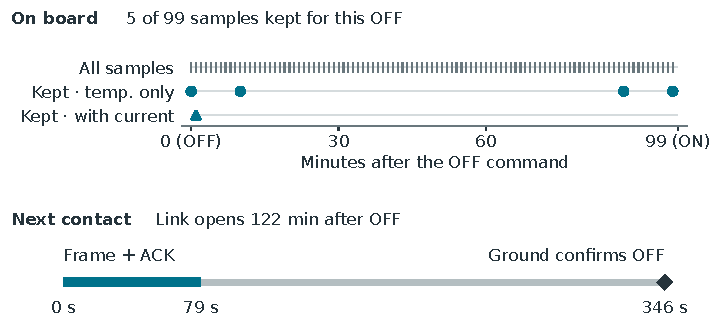
\includegraphics[width=\linewidth]{figures/workflow_trace.pdf}
\caption{Measurements selected for one OFF command and delivered at the next contact.}\label{fig:workflow}
\end{figure}
For the second OFF in Fig.~\ref{fig:workflow}, Eq.~\eqref{eq:onboard-summary} selects records at $(0, 1, 10, 88, 98)$~min after the command. One frame carries 10 records for two OFF commands. Observations (178 bytes), command context (26), framing (56) and the ACK (56) use 316 of 1\,383 available bytes at 32~bit/s. The second OFF is confirmed in time. The first has missed its deadline.


\paragraph{Comparison policies.} Fresh raw and FIFO send the newest and oldest available records first, respectively. Compact variants attach interval identifiers and self-contained command context. Thinned history retains temperature every 600~s and every current record. Fixed groups deliver observations from 600~s before until 3600~s after an OFF once that span is observed. Greedy groups rank the same fragments by a structural score per byte. Neither grouping rule sees diagnostic truth.

\paragraph{Contacts and samples.} A frozen public element set for KazSTSAT (NORAD 43783, epoch 12 November 2026, 14:08:29 UTC) gives 28 calculated windows in seven days over a model station near Astana (51.1694$^\circ$ N, 71.4491$^\circ$ E, 350~m, elevation $\geq10^\circ$). Durations are 318.1--482.8~s and end-to-start gaps 1.46--11.45~h. Each episode takes a random 24~h segment from offsets over the first six days. The periodic control has 300~s windows every 5400~s with random first start between 300 and 1800~s. These are visibility and diagnostic-stream assumptions; the mission source establishes satellite identity~\cite{kazstsat}.

Exploration uses 40 independent episodes per profile, balanced by fault presence, at 2, 4, 8, 32 and 2048~bit/s. Independent lossless validation uses 2000 new episodes per profile with an independent 0.5 probability of late failure. The protocol froze the detector, summary, seeds, endpoints and margins. Its primary grid includes three profiles, two schedules and two allocations (8 and 32~bit/s). The first 400 registered episodes per profile form a matched secondary sample for alternative policies and the 4~bit/s boundary.

\paragraph{Endpoints and inference.} Timely resolution requires a correct outcome within six hours of each OFF. Capped delay assigns missed targets six hours. Issued-error risk is the proportion of episodes with any incorrect diagnosis. Daily wire bytes cover all transmissions across 24~h; transmission continues after diagnosis. Each episode contributes the mean of its three transition outcomes. Repeated schedules and rates preserve pairing.

Equivalence to contact history requires all 36 simultaneous paired intervals (three metrics in 12 cells) inside the declared tolerances: 5 percentage points (pp) for resolution, 2~pp for episode-error risk and 900~s for capped delay~\cite{lakens2017}. At family level 0.05 the frozen protocol uses two-sided empirical Bernstein bounds for resolution and delay~\cite{maurer2009} and exact binomial bounds for the two directions of error discordance~\cite{clopper1934}. Secondary lossless intervals use 1000 paired bootstrap samples and are pointwise.

\section{Lossless Results}

\paragraph{Context and traffic.} On the exploratory KazSTSAT grid at 32~bit/s, summaries resolved 216 of 360 targets against 217 for contact history, with 41.7~s excess mean capped delay (Table~\ref{tab:explore}). Fresh compact resolved 149. The average of all 120 daily totals was 626.96 bytes for summaries versus 6390.67 for fresh compact, a saving of $100(1-626.96/6390.67)=90.2\%$. These values include framing and ACKs.
\begin{table}[!htb]\centering\small
\caption{Lossless exploratory KazSTSAT windows at 32 bit/s. All 360 OFF outcomes enter the six-hour capped delay. Daily bytes include framing, context and ACKs.}\label{tab:explore}
\begin{tabular}{@{}lrrr@{}}\toprule
Representation & Correct / 360 & Delay (h) & Bytes/day\\\midrule
Fresh raw & 80 & 5.13 & 6389\\
Fresh compact & 149 & 4.27 & 6391\\
FIFO raw & 34 & 5.69 & 6389\\
FIFO compact & 56 & 5.54 & 6394\\
Fixed groups & 184 & 4.72 & 4719\\
Greedy groups & 184 & 4.68 & 4720\\
Thinned history & 194 & 4.40 & 3833\\
Event summaries & 216 & 3.97 & 627\\
Contact full history & 217 & 3.96 & Unlimited\\
\bottomrule\end{tabular}\end{table}


\paragraph{Validation and missed deadlines.} All 36 simultaneous intervals fell within their respective margins (Table~\ref{tab:validation}). The largest upper bounds were 2.54~pp for resolution loss, 0.40~pp for excess episode-error risk and 645.8~s for delay excess. No primary episode issued an error, with a descriptive absolute-risk 95\% upper bound of 0.184\% per cell. Contact history itself resolves only 60.75--61.73\% under orbital windows, versus 99.95--100\% under periodic contacts.
\begin{table}[!htb]\centering\small
\caption{Outer limits of the three profile-specific simultaneous intervals at each setting (2000 paired episodes per profile). Positive values favor contact history. Error-risk intervals are [$-0.40$, 0.40] pp throughout.}\label{tab:validation}
\begin{tabular}{@{}lrrr@{}}\toprule
Schedule & bit/s & Resolution loss (pp) & Delay excess (s)\\\midrule
KazSTSAT & 8 & [-1.86, 2.54] & [-401.7, 534.0]\\
KazSTSAT & 32 & [-1.86, 2.54] & [-401.7, 532.9]\\
Periodic & 8 & [-1.87, 2.37] & [-401.7, 645.8]\\
Periodic & 32 & [-1.87, 2.37] & [-401.7, 645.8]\\
\bottomrule\end{tabular}\end{table}


Table~\ref{tab:attribution} explains why only 61.27\% of historical OFF outcomes were resolved. Of 6\,971 missed deadlines, only 22 were recoverable by sending unlimited history at the same contacts. The timing category has a contact overlapping the horizon but no contact starting after evidence was acquired and ending with time for diagnosis. Three nominal OFF intervals ended between sparse current samples and their thermal pairs fit both hypotheses. This post hoc partition attributes failure to the earliest limiting stage of the fixed model.

\begin{table}[!htb]\centering\small
\caption{Validation outcomes at 32 bit/s under calculated KazSTSAT windows. Indented rows partition all missed outcomes at the six-hour deadline.}\label{tab:attribution}
\begin{tabular}{@{}lrrr@{}}\toprule
Outcome & Failed OFF & Nominal OFF & All\\\midrule
OFF targets & 4\,467 & 13\,533 & 18\,000\\
Correct within six hours & 2\,769 & 8\,260 & 11\,029\\
Any incorrect decision & 0 & 0 & 0\\
No decision & 1\,698 & 5\,273 & 6\,971\\
\quad No contact overlaps the horizon & 1\,593 & 4\,876 & 6\,469\\
\quad Contact misses usable evidence & 102 & 375 & 477\\
\quad Resolved only by contact history & 3 & 19 & 22\\
\quad Continuous history insufficient & 0 & 3 & 3\\
\bottomrule\end{tabular}\end{table}


\paragraph{Budget boundary.} On the matched secondary sample at 4~bit/s, orbital-window summaries resolved 50.50--52.50\% versus 60.00--61.17\% for contact history, with 1688--1999~s excess delay. Periodic-contact summaries still resolved 99.58--100\%, yet mean excess delay reached 4441--5130~s (Fig.~\ref{fig:budget}). At 32~bit/s on the orbital schedule summaries resolved 18.75--20.83~pp more targets than fresh compact across profiles and cost 5748--5801 fewer bytes/day.
\begin{figure}[!tb]
\centering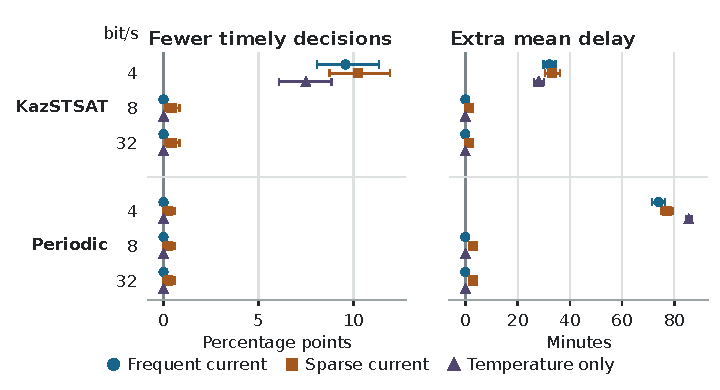
\includegraphics[width=\linewidth]{figures/budget_boundary.pdf}
\caption{Event summaries versus full history at the same contacts. Zero marks equality. Whiskers show pointwise 95\% paired bootstrap intervals.}\label{fig:budget}
\end{figure}

\section{Summary Composition and Sensor Response}

An additional matched experiment uses 360 new episodes (60 healthy and 60 with late failure per profile). Three rules share the same lossless orbital contacts, context, cache, packing and detector: endpoints alone, endpoints plus the first available current-bearing record, and the full summary. Endpoints retain any current they carry in every rule. All allocate 4, 8 or 32~bit/s and reserve 0.1~s each for selection and ground diagnosis.

A separate test at 32~bit/s introduces a first-order lag of 120~s in temperature sensing. The sensor follows a linear interpolation between successive noiseless temperatures up to acquisition. The heater, current channel, noise draws and detector are shared with zero-lag controls. Both complete-history references use the same lagged temperatures.
With zero lag, adding the first available current-bearing record improved resolution by 18.61~pp. Adding both thermal-offset selection rules gained 11.57~pp [10.37, 12.78] for 118 extra bytes/day (Table~\ref{tab:ablation}). All 125 net additional resolutions came from the temperature-only profile (97 to 222 of 360). Both current-equipped profiles matched on resolution and mean capped delay. The comparison tests the two offsets jointly. Intervals are descriptive pointwise 95\% paired percentile intervals from 5000 whole-episode resamples within profile and fault-assignment strata. At 4~bit/s the three rules resolved 253, 482, 574 targets in table order. At 8~bit/s their counts matched those at 32~bit/s.

With a 120~s sensor lag, the summary resolved 664 commands in time and full history at the same contacts resolved 607. The detector encountered conflicting evidence for 6 commands with summaries and 64 with full history. Omitting one of two contradictory readings can leave an apparently unambiguous diagnosis. The lower conflict count alone cannot establish greater diagnostic reliability. With continuous history the same detector issued a wrong decision for 65 commands, reached a correct decision at least once for 1013, and ended with a correct decision for 967.

\begin{table}[!htb]\centering\small
\caption{Summary composition on the same 1080 historical OFF commands at 32 bit/s. Correct, wrong and no-decision counts refer to the six-hour horizon. Delay is capped at six hours.}\label{tab:ablation}
\begin{tabular}{@{}rlrrrrr@{}}\toprule
Lag (s) & Records & Correct & Ever wrong & None & Delay (h) & B/day\\\midrule
0 & Endpoints & 345 & 0 & 735 & 4.78 & 490\\
0 & Endpoints + current & 546 & 0 & 534 & 4.26 & 524\\
0 & Full summary & 671 & 0 & 409 & 3.92 & 641\\
120 & Endpoints & 337 & 0 & 743 & 4.82 & 490\\
120 & Endpoints + current & 545 & 0 & 535 & 4.26 & 524\\
120 & Full summary & 664 & 0 & 416 & 3.94 & 641\\
\bottomrule\end{tabular}\end{table}


Table~\ref{tab:stress} gives the earlier model checks. Gaussian noise produced three final conflicts with full history. Plant-time-constant mismatch produced two issued errors even with continuous access. Selective delivery can hide contradictions. These exploratory conditions fall outside the baseline equivalence claim.
\begin{table}[!htb]\centering\small
\caption{Earlier one-factor stresses, 120 OFF targets per row with sparse current. $^a$Continuous full history. $^b$Summaries use orbital windows at 32 bit/s.}\label{tab:stress}
\begin{tabular}{@{}lrrrr@{}}\toprule
Condition & Final correct$^a$ & Ever wrong$^a$ & Timely$^b$ & Unknown$^b$\\\midrule
Baseline & 120 & 0 & 72 & 48\\
Current bias +0.15 A & 119 & 0 & 68 & 52\\
Gaussian noise & 117 & 0 & 73 & 47\\
Plant $\tau\times1.35$ & 115 & 2 & 71 & 49\\
\bottomrule\end{tabular}\end{table}


\section{Detection under Frame Loss}\label{sec:loss}
Figure~\ref{fig:loss} and Table~\ref{tab:loss} compare fault detection on calculated KazSTSAT contacts at 32~bit/s.
\begin{figure}[!tb]
\centering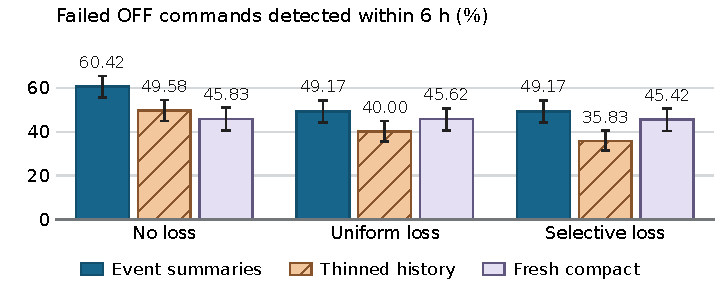
\includegraphics[width=\linewidth]{figures/loss_detection.pdf}
\caption{Six-hour fault detection on calculated KazSTSAT contacts at 32~bit/s. Whiskers show pointwise 95\% bootstrap intervals.}\label{fig:loss}
\end{figure}
\begin{table}[!htb]\centering\small
\caption{New KazSTSAT-window experiment at 32 bit/s. The raw number of correct fault decisions is out of 357 failed transitions. The primary percentage averages within episodes. Delay includes unresolved failures at six hours. Bytes/day average actual traffic over all 480 episodes.}\label{tab:loss}
\begin{tabular}{@{}llrrrr@{}}\toprule
Loss & Delivery & Correct & Detected (\%) & Delay (h) & Bytes/day\\\midrule
No loss & Event summaries & 216 & 60.42 & 3.81 & 643\\
No loss & Thinned history & 180 & 49.58 & 4.50 & 3867\\
No loss & Fresh compact & 161 & 45.83 & 4.03 & 6390\\
Uniform & Event summaries & 175 & 49.17 & 4.39 & 695\\
Uniform & Thinned history & 144 & 40.00 & 4.86 & 4013\\
Uniform & Fresh compact & 160 & 45.62 & 4.05 & 6315\\
Selective & Event summaries & 175 & 49.17 & 4.39 & 695\\
Selective & Thinned history & 129 & 35.83 & 4.98 & 4046\\
Selective & Fresh compact & 159 & 45.42 & 4.07 & 6315\\
\bottomrule\end{tabular}\end{table}

Three profiles contributed 80 healthy and 80 late-failure episodes each. The same 480 episodes ran under both schedules, two rates (8 and 32~bit/s), three representations and three link conditions. Calculated KazSTSAT contacts at 32~bit/s defined the primary comparison. This independent series retains the frozen generator, detector and selection rules.

The lossless control delivers every frame. The impaired links share a one-in-three pseudorandom erasure opportunity per contact; a selected nonempty batch loses one frame. Uniform erasure ranks all frames randomly. Selective erasure uses the same ranks but first restricts candidates to frames carrying explicit OFF context if any are present. The model sees this marker at an application boundary. Sensor values, fault state and future records remain hidden. Each attempt consumes forward bytes; a successful frame incurs a reliable 56-byte ACK. An erased frame leaves its reserved ACK slot silent. Only later contacts may resend missing evidence. Loss of the ACK after successful data reception was outside this design.

For each episode with a fault, detection is the fraction of its failed OFFs correctly identified within six hours. The estimate equally weights profile means. For the six paired method comparisons within loss conditions, 20\,000 bootstrap draws resample fault-bearing episodes within each profile jointly across conditions. Percentile limits use two-sided error probability $0.05/6$ per contrast for approximate familywise coverage.

Of 480 episodes, 240 had late faults and included 357 failed OFF commands. Summary minus thinned-history detection was 9.17 [3.75, 14.79]~pp under uniform and 13.33 [7.71, 18.96]~pp under selective erasure (adjusted paired intervals). Summary minus fresh compact was 3.54 [-3.33, 10.21] and 3.75 [-3.12, 10.42]~pp. Thinned minus fresh was -5.62 [-12.50, 1.25] and -9.58 [-16.88, -2.29]~pp. No healthy episode raised a false alarm; missed faults remained unresolved.

All 532 affected summary batches contained one frame. The two rules therefore erased the same frames, accounting for the identical 49.17\% estimates. Fresh compact had lower capped delay but transmitted roughly nine times as many bytes. On periodic contacts at 32~bit/s under uniform erasure, thinned history resolved 100.00\% of faults, fresh compact 98.54\% and summaries 96.88\%. This reversal is descriptive.


\section{Laboratory Check and Limitations}

APMonitor TCLab supplies measured heater commands and temperatures~\cite{apmonitor2021,park2020}. The first 400 observations of \texttt{initial\_models.csv} (before 400~s) were used for fitting and the next 200 for testing. The test includes one nominal OFF without current, injected fault labels or independent health certification. Two models fitted on calibration data continue into the test segment without resetting state. Held-out RMSE was 6.31~$^\circ$C for a first-order model and 0.51~$^\circ$C for a two-state lag model. Measured temperature rose by 0.80~$^\circ$C after OFF and peaked 8.98~s later (Fig.~\ref{fig:lab}). The fit cannot separate sensor inertia from plant dynamics. The 98.93~s OFF trace is too short for a 300~s pair. This example probes temperature prediction after nominal switching; it provides no fault-detection or delivery-policy validation.
\begin{figure}[!tb]
\centering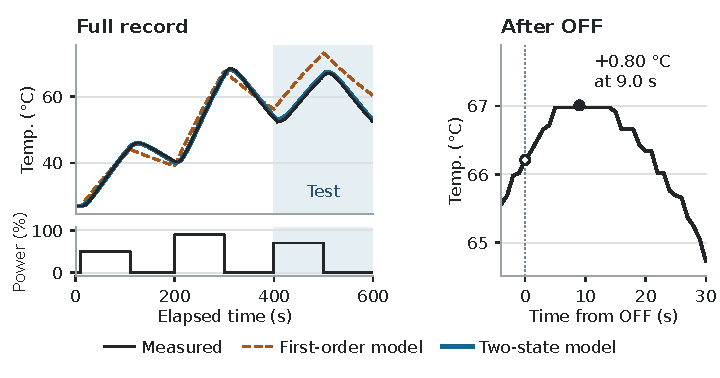
\includegraphics[width=\linewidth]{figures/lab_physics.pdf}
\caption{TCLab temperature and model predictions. The measured temperature briefly rises after heater shutdown.}\label{fig:lab}
\end{figure}

Synthetic results concern one actuator, assumed error bounds, one orbital epoch and a model station. In validation, seven full-history computations exceeded the 0.1~s reserve (maximum 0.228~s); fixing the reserve changed one first-correct reference time by less than 0.068~s and no classification. Host latency does not characterize flight hardware. Additional failures, energy use, unreliable ACKs after successful reception and within-contact adaptation remain outside the evaluated model.

\section{Conclusion}
For the fixed detector, the rolling summary met the equivalence margins for timely resolution, error risk and capped delay across all three telemetry profiles on both lossless schedules at 8 and 32~bit/s. At 4~bit/s it missed more deadlines than full history on the orbital schedule. With a working current channel, endpoints plus the first current sample matched the full summary's timely resolution count on the 32~bit/s zero-lag sample. Extra thermal samples contributed when current was unavailable. Long orbital gaps still left many deadlines unreachable even with full history. Under the uniform and selective erasure rules on the orbital schedule at 32~bit/s, summaries detected more faults in time than thinned history at lower traffic. The paired comparisons with fresh contextualized measurements were inconclusive. On the periodic schedule under uniform erasure, thinned history had the highest observed detection rate.


\paragraph{Reproducibility.} The archive \texttt{R2\_Frame\_Loss\_Research.zip} contains the code, protocols and data. \ifResearchAttached Save the ZIP from the PDF's Attachments panel. \fi Its root \texttt{README.md} explains how to verify the archived results and repeat the experiments.
\bibliographystyle{splncs04}
\bibliography{references}
\end{document}
